\documentclass[12pt]{article}
\usepackage[margin=1.0in]{geometry}

%\usepackage[utf8]{inputenc}
%\usepackage[T1]{fontenc}
%\usepackage{fixltx2e}
%\usepackage{longtable}
%\usepackage{float}
%\usepackage{wrapfig}
%\usepackage{rotating}
%\usepackage[normalem]{ulem}
%\usepackage{textcomp}
%\usepackage{marvosym}
%\usepackage{wasysym}
%\tolerance=1000

\usepackage{graphicx}
\usepackage{amsmath}
\usepackage{amssymb}
\usepackage{amsfonts}
\usepackage{bm}
\usepackage{algpseudocode}
\usepackage{hyperref}
\usepackage{booktabs}
\usepackage{listings}

\lstset{language=C}
\newcommand{\pd}[2]{\frac{\partial #1}{ \partial #2}}
\renewcommand{\v}[1]{\bold{#1}}
\setlength{\parindent}{0cm}

\title{CS 598 Final Project}
\author{Scott High and Erin Molloy}
\date{\today}

\begin{document}

\maketitle

\section{Introduction}
Molecular dynamics simulations are important for researching physical phenomena 
from the electronic structures of metals to the folding trajectories of proteins. 
In our final project, we create a performance expectation for a computationally
intensive function in a mini-application, called \href{https://github.com/exmatex/CoMD}{\texttt{CoMD}}, 
which is a code base designed to expose core features of molecular dynamics simulations
while being simple to understand and modify \cite{CoMD}. \\
 Our contributions include
\begin{itemize}
    \item [(1)] A {\bf performance expectation} for the Lennard-Jones force computate function.
    \item [(2)] Simple code {\bf modifications} which improve performance by 25-27\%.
    \item [(3)] An illustration that {\bf compiler choice} impacts compute function performance.
\end{itemize}

\section{Background}
A molecular dynamics simulation models the movements of individual particles over time. 
Particle motion is determined by Newton's well-known equation of motion, $F = ma$. 
In an $N$-particle simulation, the force acting on particle $i$ at position 
$\bm{r}_i = (x_i, y_i, z_i)$ is given by
\begin{align*}
    \textbf{F}_i = m_i \ddot{\bm{r}}_i = -\frac{\partial}{\partial \bm{r}_i} U(\bm{r}_1, \dots, \bm{r}_N)
\end{align*}
where $U$ is the potential energy from particle-particle interactions \cite{Intro}.
The resulting system of first order ODEs is integrated to find the positions of particles
at each time step. The \texttt{CoMD} mini-application computes force using the truncated 
Lennard-Jones potential, where the the potential between a pair of particles, call $i$ and $j$,
is given by
\begin{align}
U_{LJ_{trunc}}(r_{ij}) = 
\left\{ \begin{array}{l c} 
     U_{LJ}(r_{ij}) - U_{LJ}(r_c) & r_{ij} \le r_c \\
     0 & r_{ij} > r_c
    \end{array} \right.
\end{align}
where
\begin{align}
    U_{LJ}(r) = 
    4 \epsilon \left\{ \left(\frac{\sigma}{r}\right)^{12} - 
    \left(\frac{\sigma}{r}\right)^6 \right\}
\end{align}
is the Lennard-Jones potential,
\begin{align}
    r_{ij} = \sqrt{(x_i - x_j)^2 + (y_i - y_j)^2 + (z_i - z_j)^2}, 
\end{align}
is the distance between particles and $r_c = 2.5 \sigma$ is the cut-off radius for 
particle-particle interactions. In particular, the cut-off radius defines a sphere with
volume within which pair potentials must be computed. Material parameters 
$\epsilon$ and $\sigma$ are the potential well depth and distance at which the 
pair potential becomes zero, respectively \cite{Wiki}. 

\section{Performance baseline}
\texttt{CoMD} includes a default simulation of Copper atoms in a face-centered 
cubic (FCC) lattice with a fully periodic domain and a spacing of $3.615 \text{ \AA}$.
Material parameters are defined as $\epsilon = 0.167 \text{ eV}$ and $\sigma = 2.315 \text{ \AA}$ 
\cite{CoMD}. Thus, there exist
\begin{align}
     \bigg( \frac{4}{3} \pi (2.5 \cdot 2.315)^3 \text{ \AA}^3 \bigg) \times
     \bigg( \frac{4 \text{ particles}}{3.615 \text{ \AA} \times 3.615 \text{ \AA} \times 3.615 \text{ \AA}} \bigg)
     \approx 69 \text{ particles}
\end{align}
within the cut-off radius of each particle at lattice initialization. \\

 In a scaling study, we use these default parameters for temperatures of 
0, 600, and 3000 K. Strong scaling studies with 16,384,000 atoms are
performed on 64, 512, and 4096 processors. Weak scaling studies are
performed with 32000 atoms per processor for 1, 8, 64, 512, and 4096 
processors. Table 1 shows the difference in runtimes for the force compute
function and the halo exchange. As the former dominated total runtime, 
we target the force computation function in order to improve the overall 
performance. \\

 In our performance baseline, we use default parameters with a temperature of 
0 K so that particles remain in their initial positions throughout the simulation.
This enables us to model the number of particle-particle interactions as the 
constant value. Figure 1 shows the runtimes for the force computation on 
a single processor with the problem size increasing from 4000 to 4000000 
atoms. Runtimes increase linearly in the number of atoms. \\

 All scaling and baseline results are obtained on Blue Waters by compiling 
\texttt{CoMD} with the default Cray compiler (optimization flags: \texttt{-g -O3}).

\begin{table}[h!]
\centering
\begin{tabular}{c c | c c | c c}
\toprule
& \multicolumn{1}{c}{} & \multicolumn{2}{c}{Strong scaling} & \multicolumn{2}{c}{Weak scaling} \\
\cmidrule(r){3-4} \cmidrule(r){5-6}
\multicolumn{1}{c}{} & \multicolumn{1}{c}{}  & \multicolumn{1}{c}{force} & \multicolumn{1}{c}{halo} & \multicolumn{1}{c}{force} & \multicolumn{1}{c}{halo} \\
\multicolumn{1}{c}{temperature} & \multicolumn{1}{c}{\# ranks} & \multicolumn{1}{c}{computation} & \multicolumn{1}{c}{exchange} & \multicolumn{1}{c}{computation} & \multicolumn{1}{c}{exchange} \\
\midrule
 & 1 & - & - & 5.1e-1/97.4\% & - \\ 
& 8 & - & - & 6.2e-1/96.5\% & 1.2e-3/0.2\% \\ 
$T = 0 K$ & 64 & 4.8e-0/96.8\% & 2.2e-2/0.4\% & 6.2e-1/96.3\% & 3.9e-3/0.6\% \\ 
& 512 & 6.2e-1/85.9\% & 8.2e-2/11.4\% & 6.2e-1/91.4\% & 5.9e-3/0.9\% \\ 
& 4096 & 8.3e-2/72.3\% & 1.8e-2/15.7\% & 6.2e-1/91.9\% & 9.0e-3/1.3\% \\ 
\midrule
 & 1 & - & - & 5.0e-1/97.4\% & - \\ 
& 8 & - & - & 6.1e-1/96.4\% & 1.4e-3/0.2\% \\ 
$T = 600 K$ & 64 & 4.8e-0/94.9\% & 9.2e-2/1.8\% & 6.1e-1/96.2\% & 3.6e-3/0.6\% \\ 
& 512 & 6.1e-1/95.9\% & 5.7e-3/0.9\% & 6.1e-1/95.9\% & 5.9e-3/0.9\% \\ 
& 4096 & 8.1e-2/67.9\% & 3.6e-3/3.0\% & 6.1e-1/92.0\% & 9.1e-3/1.4\% \\ 
\midrule
 & 1 & - & - & 5.0e-1/97.3\% & - \\ 
& 8 & - & - & 6.3e-1/96.5\% & 1.0e-3/0.2\% \\ 
$T = 3000 K$ & 64 & 4.7e-0/96.7\% & 2.3e-2/0.5\% & 6.0e-1/96.2\% & 4.2e-3/0.7\% \\ 
& 512 & 6.0e-1/95.9\% & 6.1e-3/1.0\% & 6.0e-1/95.9\% & 6.3e-3/1.0\% \\ 
& 4096 & 8.1e-2/66.3\% & 3.0e-3/2.4\% & 6.1e-1/96.4\% & 9.6e-3/1.5\% \\ 
\bottomrule
\end{tabular}
\caption{Scaling Studies (seconds spent in function/percentage of total runtime)}
\end{table}

% \begin{figure}[h!]
%     \centering
%     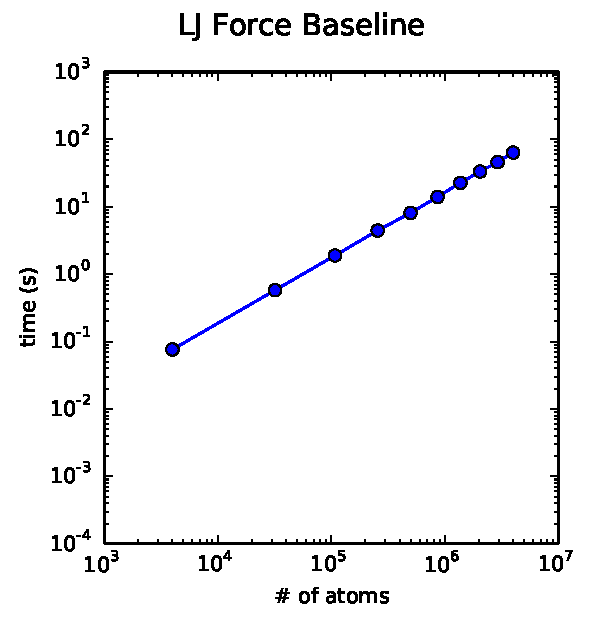
\includegraphics[width=0.45\textwidth]{../figs/baseline_forceLJ.pdf}
%     \caption{Time spent in force computation function on a single processor}
% \end{figure}

\section{Performance model}
All analysis assumes a one-level cache model and approximates read and write 
times as equal.  The constants used in the performance expectations are determined 
by the processor clock rate (2.3 GHz) and the results of the \texttt{STREAM} benchmark 
on Blue Waters. \\

\subsection{Computation-based performance model}
 Our performance model is based on the cost of updating variables associated
with particle $i$ due to interactions with each of it's $n$ neighboring atoms, $j$. Specifically,
the potential energy $U_{LJ}$ between the pair of atoms is computed as
\begin{align}
    U_{LJ}(r_{ij}) = A\left(\frac{1}{r_{ij}}\right)^{6}\left\{ \left(\frac{1}{r_{ij}}\right)^{6} - 1 \right\},           
\end{align}            
and the resulting force $\textbf{F} = (F_x, F_y, F_z)$ is computed as
\begin{align}
    \textbf{F}(r_{ij}) &= - U'_{LJ}(r_{ij})\hat{r}_{ij} \notag\\
        &= 24 \frac{\epsilon}{r_{ij}} \left\{ 2 \left(\frac{\sigma}{r_{ij}}\right)^{12}
              - \left(\frac{\sigma}{r_{ij}}\right)^6 \right\} \hat{r}_{ij} \notag\\
        &=  A \frac{1}{r_{ij}^2} \left(\frac{1}{r_{ij}}\right)^{6} \left\{ 2 \left(\frac{1}{r_{ij}}\right)^{6}
              - 1 \right\} \textbf{r}_{ij},
\end{align}
where $N$ is the total number of particles in the simulation, $n$ is the number of neighboring
particles, that is, particles within a sphere defined by the cut-off radius, $r_c$. In addition,
the total energy of the system $E_{tot}$, computed as
\begin{align}
    E_{tot} &= \sum_{ij} U_{LJ}(r_{ij}),
\end{align}
is updated within the innermost loop of the compute function. The resulting cost is
\begin{itemize}
\item[(A)] 3 loads to get particle $i$'s position, $r_i = (x_i, y_i, z_i)$
\item[(B)] For each particle $j$ where $r_{ij}<r_c$
  \begin{enumerate}
    \item 3 loads to get particle $j$'s position, $r_j = (x_j, y_j, z_j)$
    \item 3 subtractions, 3 multiplications, 2 additions, and 1 division to calculate $\frac{1}{r_{ij}^2}$ 
    \item 3 multiplications to calculate $\left(\frac{1}{r_{ij}^2}\right)^3 = \left(\frac{1}{r_{ij}}\right)^6$
    \item 2 subtractions and 2 multiplications to calculate the potential $U_{LJ}$  
             where 1 subtraction is for cutoff potential
    \item 3 multiplications and 1 subtraction to calculate magnitude of the force, $F(r_{ij})$ (equation 6)
    \item 3 multiplications and 3 additions to calculate and update the force vector, $\textbf{F}$
  \end{enumerate}
\item[(C)] 1 write to save $U_{LJ}$, assuming the $U_{LJ}(r_{ji})$ term is saved for free
\item[(D)] 3 writes to save $\textbf{F} = (F_x, F_y, F_z)$
\item[(E)] 1 addition to update $E_{tot}$ (equation 7)
\end{itemize}
The total cost is then
\begin{align}
    N\bigg(A+\frac{nB}{2}\bigg)+C+D+E,
\end{align}
where the factor of $1/2$ accounts for double counting particles in pairwise interactions, 
that is, the interaction between particle $i$ and particle $j$ is the same as the interaction 
between particle $j$ and particle $i$ making it unnecessary to compute both interactions. \\

 Let $c$ be the cost of a floating point operation, $w$ be the cost of a write, 
and $r$ be the cost of a read. Then the cost can be approximated as
\begin{equation}
    N \left(\frac{n}{2} \left(26 c + 3 w\right) + 3 w\right) + c + 4 r,
\end{equation}
which reduces to
\begin{equation}
  N \left(\frac{n}{2} \left(26 c + 3 m\right) + 3 m\right) + c + 4 m
  \label{eqn:perf-model}
\end{equation}
assuming equal read and write times, call $m$. Specifically, we
approximate $c = 4.35\times10^{-10}\;\text{flops}/s$ using the
processor clock rate, $m = 1.43\times10^{-9}\;\text{B}/s$ using the
STREAM benchmark on Bluewaters, and $n = 69$ from the known cut-off
radius and lattice parameters (equation 4).  The results of this
performance model are shown in figure \ref{fig:perf-models} for
increasing $N$. Although both our results and the computation-based
performance model scale linearly with the number of atoms, our
performance expectation is nearly 2 orders of magnitude less than our
results!

% \begin{figure}[h!]
%   \centering
%   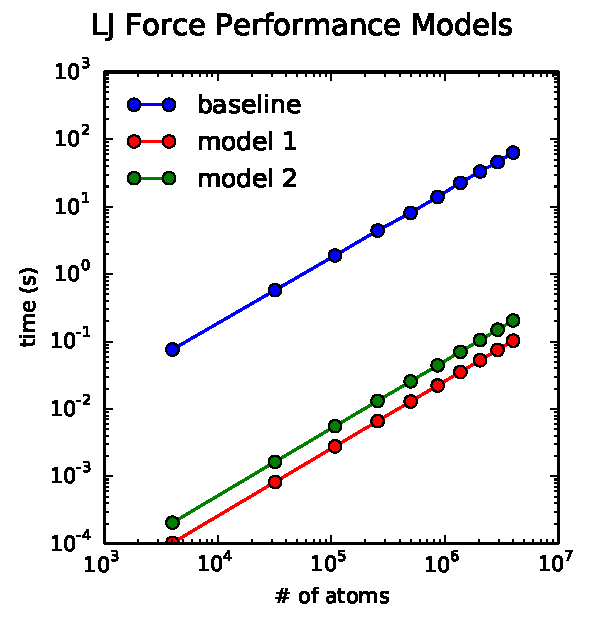
\includegraphics[width=0.45\textwidth]{../figs/perfmodel_forceLJ.pdf}
%   \caption{Computation-based performance model and baseline results}
%   \label{fig:comp-baseline}
% \end{figure}
\begin{figure}[h!]
  \centering
  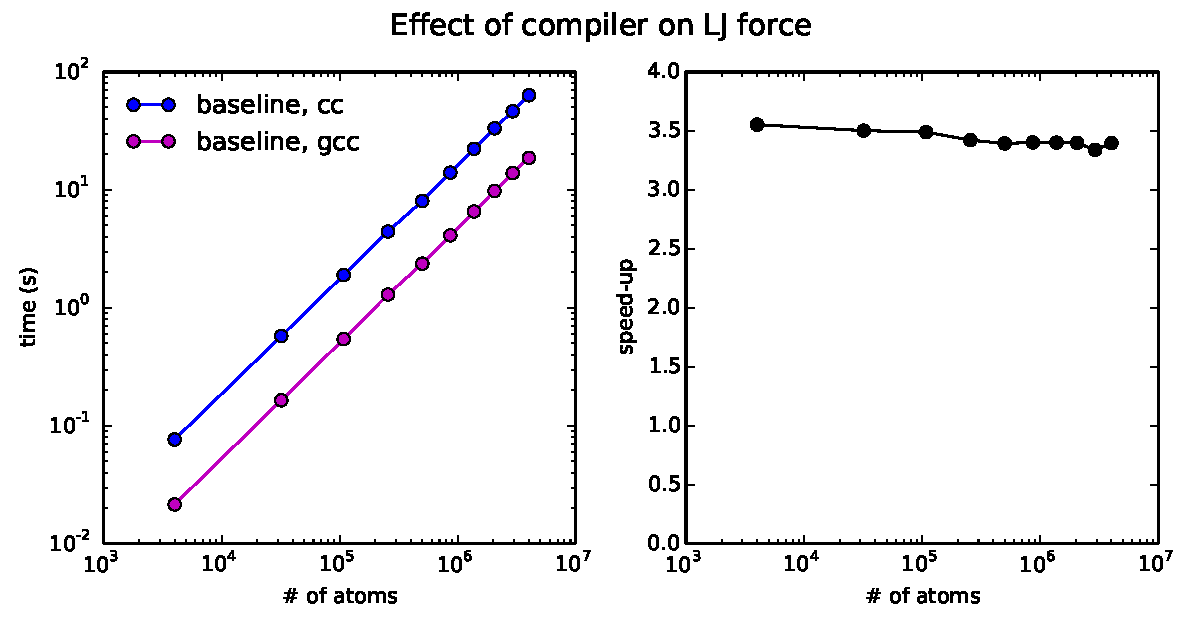
\includegraphics[width=0.45\textwidth]{../figs/compiler_forceLJ.pdf}
  \caption{Performance models and baseline results}
  \label{fig:perf-models}
\end{figure}

\subsection{Implementation-based model}
The computation-based performance model represents a best case scenario 
for the number of operations required to compute the inter-particle forces. 
To better understand our baseline results, we also develop a performance model 
that captures the features of the algorithm's implementation. \\

 The data structure used for storing the computational particles is a
struct of linear C arrays. Each linear array is divided into equal sized sections which 
store information for particles in a region of the simulation domain. 
Section size is the maximum number of particles per region of space, 
and does not change throughout the simulation. 
This ordering of particles is used to efficiently determine, which particle pairs are within 
the cutoff radius. \\

 However, this still requires work to ``check'' whether a particle 
is within the cut-off radius. Specifically, the inter-particle distance is computed as
\begin{align*}
    \| \bm{r}_i - \bm{r}_j\|_2^2,
\end{align*}
which requires an additional 3 reads, 3 subtractions, 3 multiplications, and 2 additions.
If we denote the number of particles checked, which are not within the sphere defined 
by $r_c$, as $k$, then our performance model can be updated
\begin{equation}
  N \left(\frac{n}{2} \left(26 c + 3 m\right)+\frac{k}{2} \left(8 c + 3 m\right) + 3 m\right) + c + 4 m
  \label{eqn:perf-model-nk}
\end{equation}
In addition, the actual implementation does not compute interactions
and distance checks once but rather does so for each particle. This
doubles the number of interactions and distance checks in our the
performance model \ref{eqn:perf-model-nk} to give
\begin{equation}
  N \left(n \left(26 c + 3 m\right)+k \left(8 c + 3 m\right) + 3 m\right) + c + 4 m
  \label{eqn:perf-model-2n2k}
\end{equation}
The results of these implementation-based performance model are shown
in figure \ref{fig:perf-models} for increasing $N$. These
implementation-based performance models scale linearly with the number
of atoms and appear much closer to our experimental results; however,
our performance expectation is still nearly an order of magnitude less
than our baseline.

\section{Compiler choice}
The baseline results using the Cray compiler compare poorly with the
performance models as shown in figure \ref{fig:perf-models}. We were
unable to determine why the Cray compiler has such poor performance
and obtained an additional baseline using the \texttt{CoMD} code
compiled with gcc 4.7.1. This compiler change alone resulted in a 3.5
times speed-up. The gcc baseline and performance models are also shown
in figure \ref{fig:perf-models}. From this we see that our
implementation based performance model is consistent with the baseline
run using the gcc compiler.

% \begin{figure}[h!]
%   \centering
%   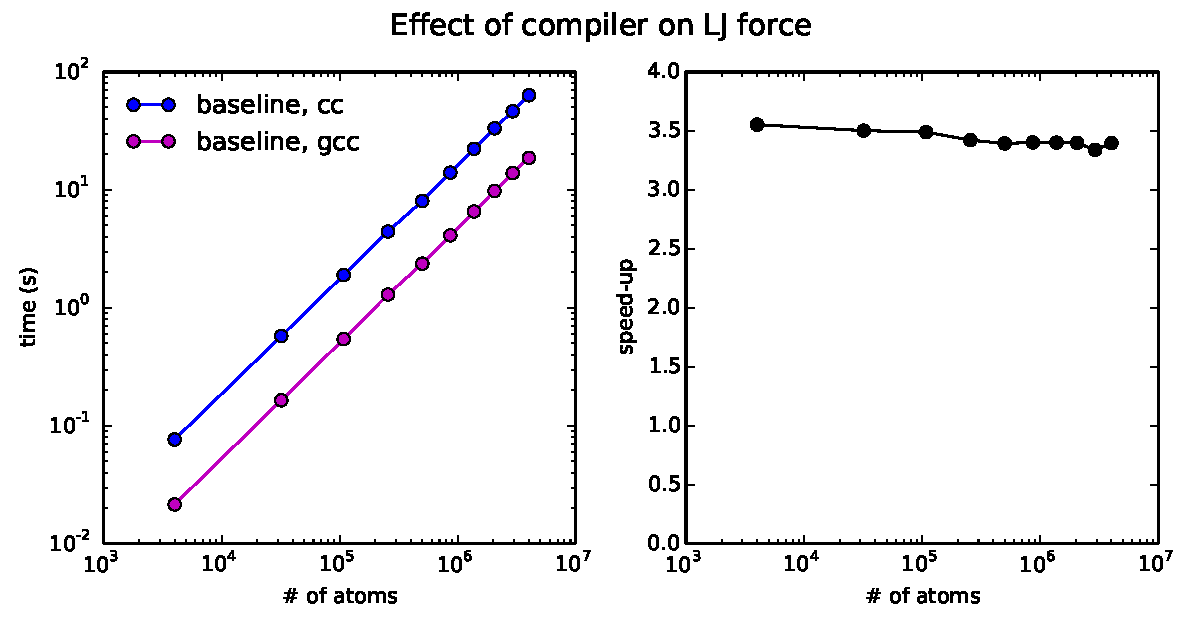
\includegraphics[width=0.9\textwidth]{../figs/compiler_forceLJ.pdf}
%   \caption{Effects of compiler choice}
%   \label{fig:comp-choice}
% \end{figure}

\section{Modifications}
\label{sec:mods}

\begin{figure}[h!]
  \centering
  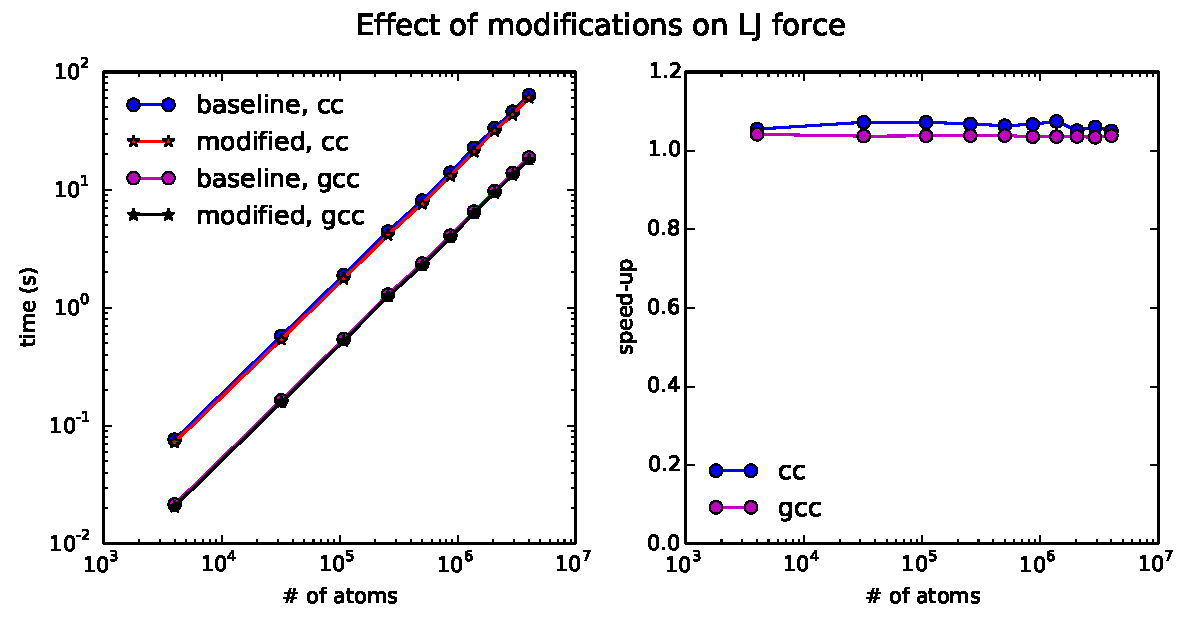
\includegraphics[width=0.9\textwidth]{../figs/modified_forceLJ.pdf}
  \caption{Runtime and speedups from the modifications described in
   section \ref{sec:mods}}
   \label{fig:mod-force}
\end{figure}

The performance baseline revealed a large discrepancy between our
performance model and experimental results for the Cray compiler. We
have focused our modifications on attempting to improve the results
using the Cray compiler. The results using the gcc compiler agree well
with our performance model, and further improvements would require
changes to the underlying data structures or a complete rewrite of the
force calculation routines, both of which are beyond the scope of this
project. The results from our modifications are shown in figure
\ref{fig:mod-force}.

 The force compute function uses a large number of pointer dereferences
to access the arrays storing particle information. For example, accessing the $m^{th}$ 
component of the position vector corresponding to particle $i$ requires two pointer 
dereferences: \texttt{s->atoms->r[iOff][m]}. From the code report generated by the Cray 
compiler, it was clear that these dereferences were being done {\bf each time} the
pointers were accessed in the innermost loop of the force calculation. 
Thus, a simple optimization is to dereference these pointers outside the computation 
loops (\ref{apd:code-changes}). \\

 In addition, small loops over a set of 3 real variables are frequently used to
work with position $\bm{r}$ and force $\textbf{F}$ vectors. Not only does this prevent the pipelining
of instructions, but this also requires additional clock cycles to execute branch instructions.
Accordingly, we unrolled all of these loops by hand. The inner loop of the force calculation 
routine is shown before and after optimization in appendix \ref{apd:code-changes}. \\

 The Cray compiler reports tell us that no vectorization
occurs during the force calculation. After some investigation, we
determined that this is, in fact, the correct behavior as the data
structure does not guarantee that pointers to arrays associated with
particle data are not aliased.  Specifically, aliasing does occur when
calculating the interactions between particles within the same
cell. We considered modifying the data structure to remove aliasing;
however, we decided
that such substantial modifications were beyond the scope of this project. \\

% \begin{figure}[h!]
%   \centering
%   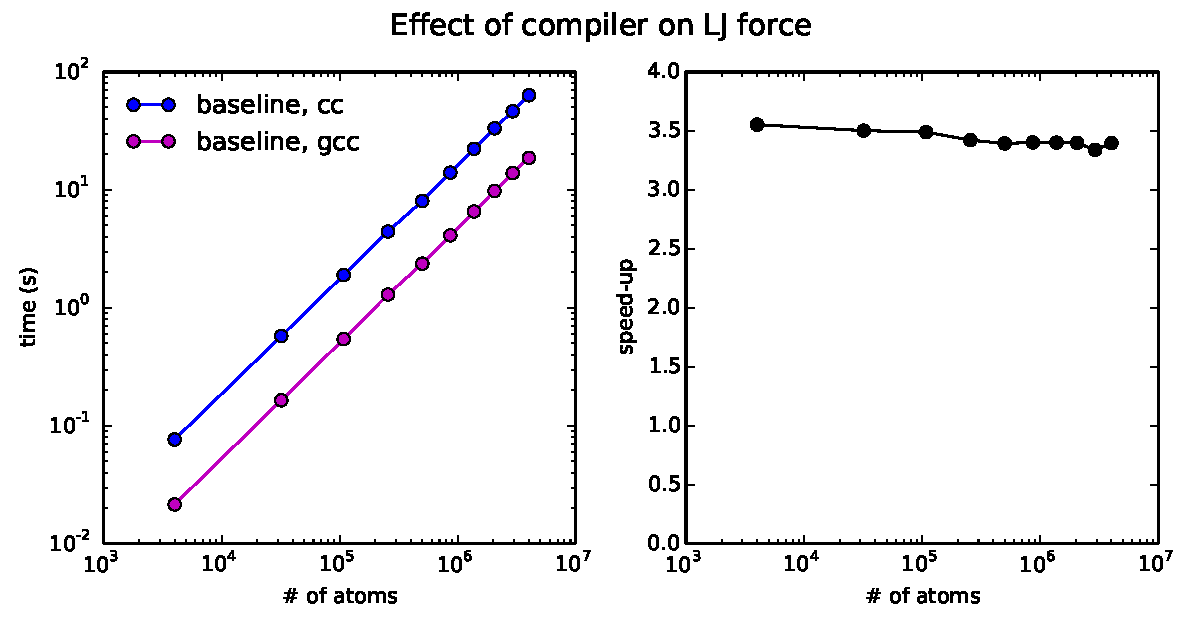
\includegraphics[width=0.9\textwidth]{../figs/compiler_forceLJ.pdf}
%   \caption{Runtime and speedups from the modifications described in
%    section \ref{sec:mods}}
%    \label{fig:mod-force}
% \end{figure}

 Another potential improvement considered was changing the order of
particles within a cell to improve memory access patterns. However, as the
current implementation already sorts the particles within a cell regularly, it is unlikely 
that we could substantially improve upon its current performance. \\

 The above modifications led to a 1.24-1.27 speed-up using
the Cray compiler; however, runtimes are still much higher than our
performance expectations. With these changes the gcc compiler only
experienced a speed-up of 1.04-1.05. It is likely that the gcc
compiler had already made similar optimizations, so our manual editing
made only minor improvements.
% ; however, we have not been able
% to identify the causes of the remaining discrepancy between compilers
% as both compiler reports show no vectorization.

% \begin{figure}[h!]
%   \centering
%   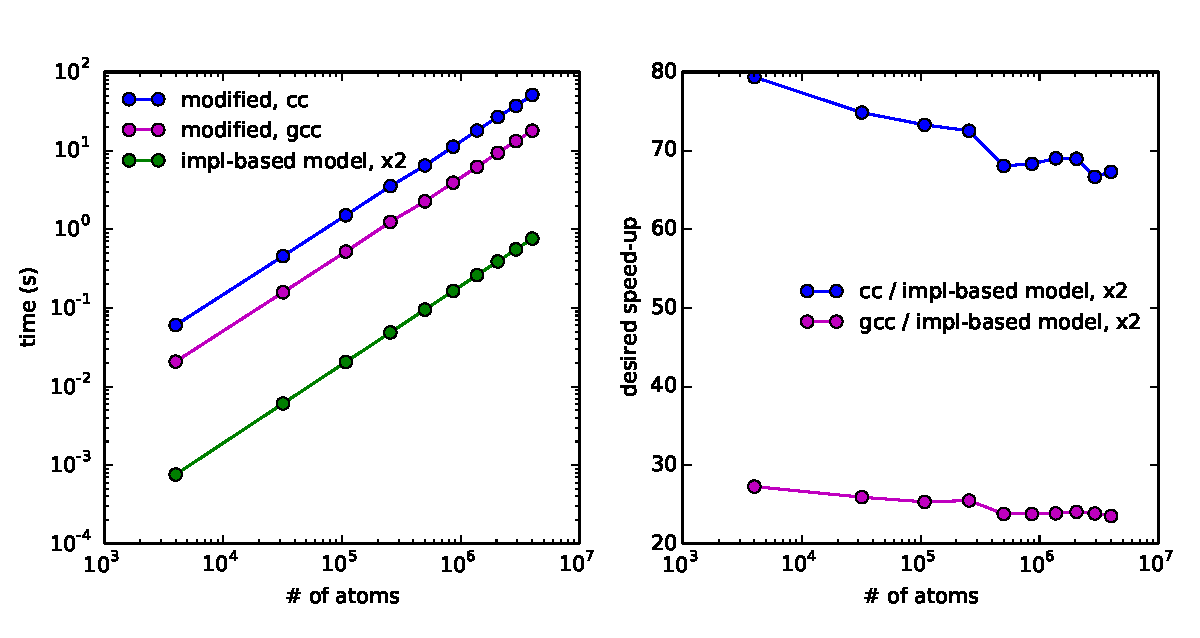
\includegraphics[width=0.9\textwidth]{../figs/futurework_forceLJ.pdf}
%   \caption{Desired speed-ups}
% \end{figure}

\section{Conclusion}
 In summary, we ran scaling studies and profiled the \texttt{CoMD} code base to 
determine a routine that could be targeted to enhance performance. We then created a 
{\bf performance expectation} for the Lennard-Jones force compute function and used this performance 
model to make modifications to this computationally intensive routine. We obtained speed-ups of
\#-\#; however, the biggest differences in performance were due to the choice of compiler. \\
Finally, we adapted our performance expectation to include implementation details, which could allow 
others to determine how changing the data structure to reduce accesses to particles outside 
the cut-off radius would impact performance before spending time implementing such substantial changes 
to \texttt{CoMD}.

\begin{thebibliography}{}
    \bibitem{CoMD} ADD ME
    \bibitem{Intro} Allen, Michael P. Introduction to Molecular Dynamics Simulation. 
      {\it Computational Soft Matter: From Synthetic Polymers to Proteins, Lecture Notes}, 
      Norbert Attig, Kurt Binder, Helmut Grubmuller, Kurt Kremer (Eds.),
      John von Neumann Institute for Computing, Julich,
      NIC Series, Vol. 23, ISBN 3-00-012641-4, pp. 1-28, 2004.
      \bibitem{Wiki} \url{http://en.wikipedia.org/wiki/Lennard-Jones_potential}
\end{thebibliography}

\appendix
\section{Code changes}
\label{apd:code-changes}
The changes made to the inner loop in the force cacluation are shown
here.
\subsection{Initial Inner Force Loop}
\begin{lstlisting}
  real_t dr[3];
  int jId = s->atoms->gid[jOff];  
  if (jBox < s->boxes->nLocalBoxes && jId <= iId )
  continue; // don't double count local-local pairs.
  real_t r2 = 0.0;
  for (int m=0; m<3; m++)
  {
    dr[m] = s->atoms->r[iOff][m]-s->atoms->r[jOff][m];
    r2+=dr[m]*dr[m];
  }

  if ( r2 > rCut2) continue;

  r2 = 1.0/r2;
  real_t r6 = s6 * (r2*r2*r2);
  real_t eLocal = r6 * (r6 - 1.0) - eShift;
  s->atoms->U[iOff] += 0.5*eLocal;
  s->atoms->U[jOff] += 0.5*eLocal;

  if (jBox < s->boxes->nLocalBoxes)
  ePot += eLocal;
  else
  ePot += 0.5 * eLocal;

  real_t fr = - 4.0*epsilon*r6*r2*(12.0*r6 - 6.0);
  for (int m=0; m<3; m++)
  {
    s->atoms->f[iOff][m] -= dr[m]*fr;
    s->atoms->f[jOff][m] += dr[m]*fr;
  }
\end{lstlisting}

\subsection{Optimized Inner Force Loop}
\begin{lstlisting}
  real_t dr[3];
  int jId = gid[jOff];  
  if (jBox < nLocalBoxes && jId <= iId )
  continue; // don't double count local-local pairs.

  real_t r2 = 0.0;
  dr[0] = r_iOff[0]-r[jOff][0];
  r2+=dr[0]*dr[0];
  dr[1] = r_iOff[1]-r[jOff][1];
  r2+=dr[1]*dr[1];
  dr[2] = r_iOff[2]-r[jOff][2];
  r2+=dr[2]*dr[2];

  if ( r2 > rCut2) continue;

  r2 = 1.0/r2;
  real_t r6 = s6 * (r2*r2*r2);
  real_t eLocal = r6 * (r6 - 1.0) - eShift;
  U[iOff] += 0.5*eLocal;
  U[jOff] += 0.5*eLocal;

  if (jBox < nLocalBoxes)
  ePot += eLocal;
  else
  ePot += 0.5 * eLocal;

  real_t fr = - 4.0*epsilon*r6*r2*(12.0*r6 - 6.0);
  f_iOff[0] -= dr[0]*fr;
  f[jOff][0] += dr[0]*fr;
  f_iOff[1] -= dr[1]*fr;
  f[jOff][1] += dr[1]*fr;
  f_iOff[2] -= dr[2]*fr;
  f[jOff][2] += dr[2]*fr;
\end{lstlisting}

\end{document}
